%==============================================================

\chapter{Results}\label{bds2}

In the last chapter of the thesis the results concerning the quality of the recommendations are shown. At the end of the chapter the work of the thesis is summarized and the open task for future work are outlined. 

\section{Objective evaluation}

\subsection{feature quality}\label{featqual}

This section analyzes the results from the similarity analysis to find out how the distances from different feature sets are correlated to each other and how they are distributed over the unit interval $[0,1]$.

\begin{figure}[htbp]
	\centering
	\framebox{\parbox{1\textwidth}{ 			
			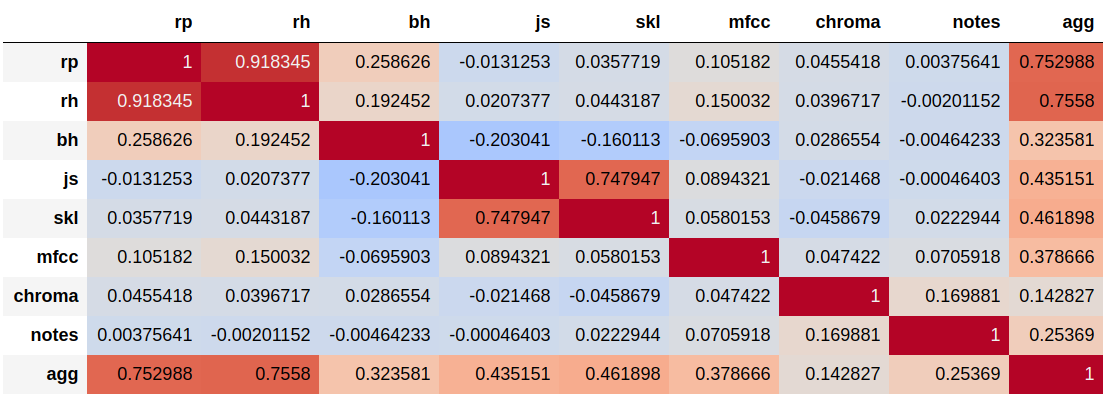
\includegraphics[scale=0.4]{Images/SparkFeat/corr_95_1517.png}	
	}}
	\caption{correlation 95 songs, 19 genres (5 each), 1517 artists}
	\label{fig:corr2}
\end{figure}


\noindent To analyze this, a test dataset consisting of distances coming from the Spark framework had to be created. 95 songs (five songs for every genre) were randomly chosen from the 1517 artists dataset and the distances to all other songs of the 1517 artists dataset were calculated. The dataset contains 3180 songs evenly distributed over 19 different genres (see figure \ref{1517dist}). The sampling of distances from different genres is important for the analysis of the distribution of the distances, because the distances vary, depending on where in the feature space the actual song is located. A song taken from the edge of the distribution of the feature space will end up with different distances than a song taken from the center. 
%For 95 song request that results in eight very large vectors containing the distances of song pairs. This large set of distances is then analyzed. 
Figure \ref{fig:corr2} shows the correlation of the distances from the various feature types. The eight different distances for each song pair are summed up into one new combined distance (following formula \ref{eq:distance} with all weights $w = 1$ ). This combined distance is labeled as "agg" in the following plots.
\noindent The correlation of a feature type with the overall distance is a sign of the impact of the feature type on the overall distance from the weighted sum. But because not all distances are equally distributed over the unit interval the different feature types have different impacts on the sum of distances. This problem was already mentioned in section \ref{distsc} and section \ref{sparkskl}. Figure \ref{fig:cumdist} shows how the distances are distributed with the cumulative histograms over the unit interval. It is clearly visible that the cross-correlation distances are not evenly distributed. In section \ref{distsc} a few proposals were already given how this problem could be solved in the future. 

\begin{figure}[htbp]
	\centering
	\framebox{\parbox{1\textwidth}{ 				
			\begin{subfigure}{.495\textwidth}
				\centering     
				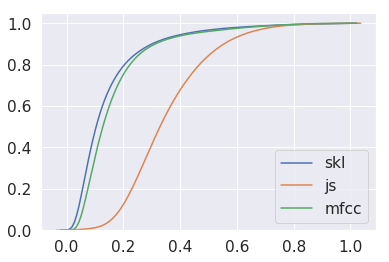
\includegraphics[scale=0.5]{Images/SparkFeat/cum1.png}
				\caption{cumulative distribution 1}
				\label{cum1}
			\end{subfigure}%	
			\begin{subfigure}{.495\textwidth}
				\centering    
				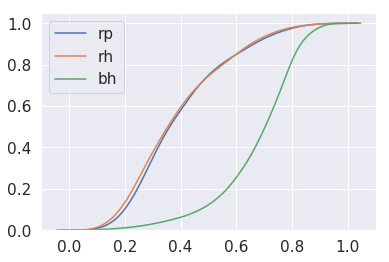
\includegraphics[scale=0.5]{Images/SparkFeat/cum2.png}
				\caption{cumulative distribution 2}
				\label{cum2}
			\end{subfigure}
			
			\begin{subfigure}{.495\textwidth}
				\centering     
				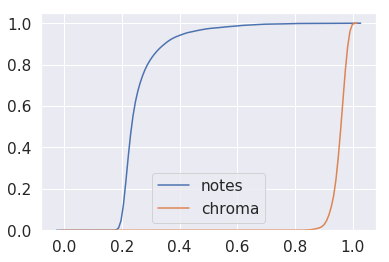
\includegraphics[scale=0.5]{Images/SparkFeat/cum3.png}
				\caption{cumulative distribution 3}
				\label{cum3}
			\end{subfigure}%		
			\begin{subfigure}{.495\textwidth}
				\centering    
				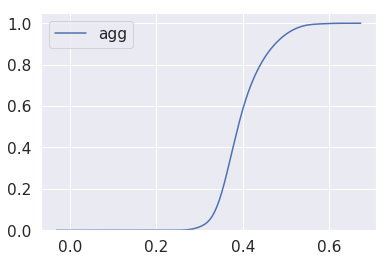
\includegraphics[scale=0.5]{Images/SparkFeat/cum4.png}
				\caption{cumulative distribution 4}
				\label{cum4}
			\end{subfigure}	
	}}
	\caption{Cumulative distributions}
	\label{fig:cumdist}
\end{figure}
\FloatBarrier

\noindent As mentioned in section \ref{sparkskl} the SKL divergence was also prone to outliers and had issues when scaling distances to the unit interval. The solution was to filter out all song pairs with an SKL divergence larger than a certain threshold before scaling the distances. If this filter operation is left out nearly all distances calculated with the symmetric Kullback-Leibler divergence are close to zero after the scaling. The impact can be seen in figure \ref{fig:sklsc} and figure \ref{fig:corr}

\begin{figure}[htbp]
	\centering
	\framebox{\parbox{1\textwidth}{ 
	\begin{subfigure}{0.5\textwidth}
		\centering
		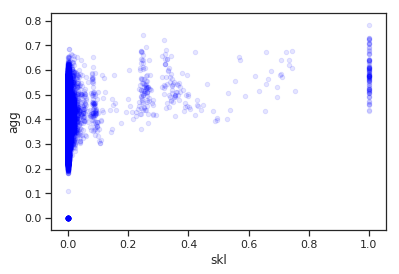
\includegraphics[scale=0.5]{Images/SparkFeat/skl_unscaled.png}
		\captionof{figure}{SKL unscaled}
		\label{scklusc}
	\end{subfigure}
	\begin{subfigure}{0.5\textwidth}
		\centering
		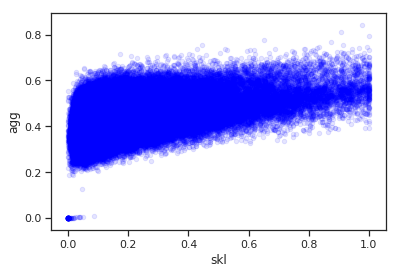
\includegraphics[scale=0.5]{Images/SparkFeat/skl_scaled.png}
		\captionof{figure}{SKL scaled}
		\label{scklsc}
	\end{subfigure}%
	}}
	\caption{Correlation of features}
	\label{fig:sklsc}
\end{figure}

\noindent If the outliers are not filtered, the correlation between the distances of the different feature types change drastically. The correlation of the unfiltered SKL distances with the combined distance ("agg") decreases significantly (see figure \ref{fig:corr}). Interestingly also the correlation of the Jensen-Shannon like divergence and the combined distance ("agg") is dropping. 
A possible explanation could be that the SKL and JS distances are indeed highly correlated but due to the bad scaling the SKL has no impact on the overall distance. The results from the JS divergence alone are not able to impact the weighed sum of the combined distance in the same way, both features together could. 

\begin{figure}[htbp]
	\centering
	\framebox{\parbox{1\textwidth}{
	\begin{subfigure}{0.5\textwidth}
		\centering
		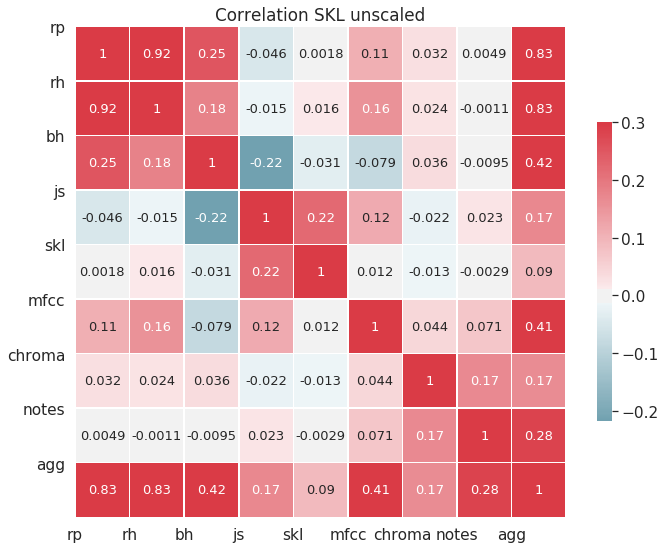
\includegraphics[scale=0.33]{Images/SparkFeat/skl_corr_unscaled.png}
		\captionof{figure}{SKL unscaled}
		\label{corrusc}
	\end{subfigure} 
	\begin{subfigure}{0.5\textwidth}
		\centering
		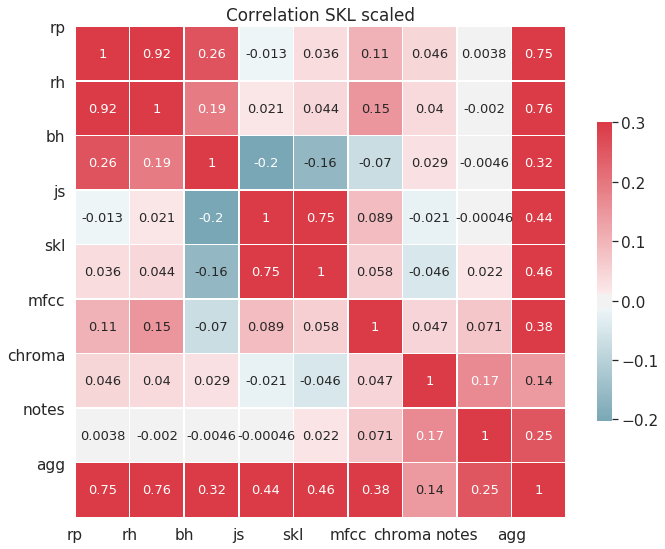
\includegraphics[scale=0.33]{Images/SparkFeat/skl_corr_scaled.png}
		\captionof{figure}{SKL scaled}
		\label{corrsc}
	\end{subfigure}%
	}}
	\caption{Correlation of features}
	\label{fig:corr}
\end{figure}
\FloatBarrier

\noindent The last plot (figure \ref{fig:corr3}) shows the full scatter matrix of the various distances. The main diagonal shows the histogram of the 

\ref{fig:corr3}
\begin{figure}[htbp]
	\centering
	\framebox{\parbox{1\textwidth}{ 			
			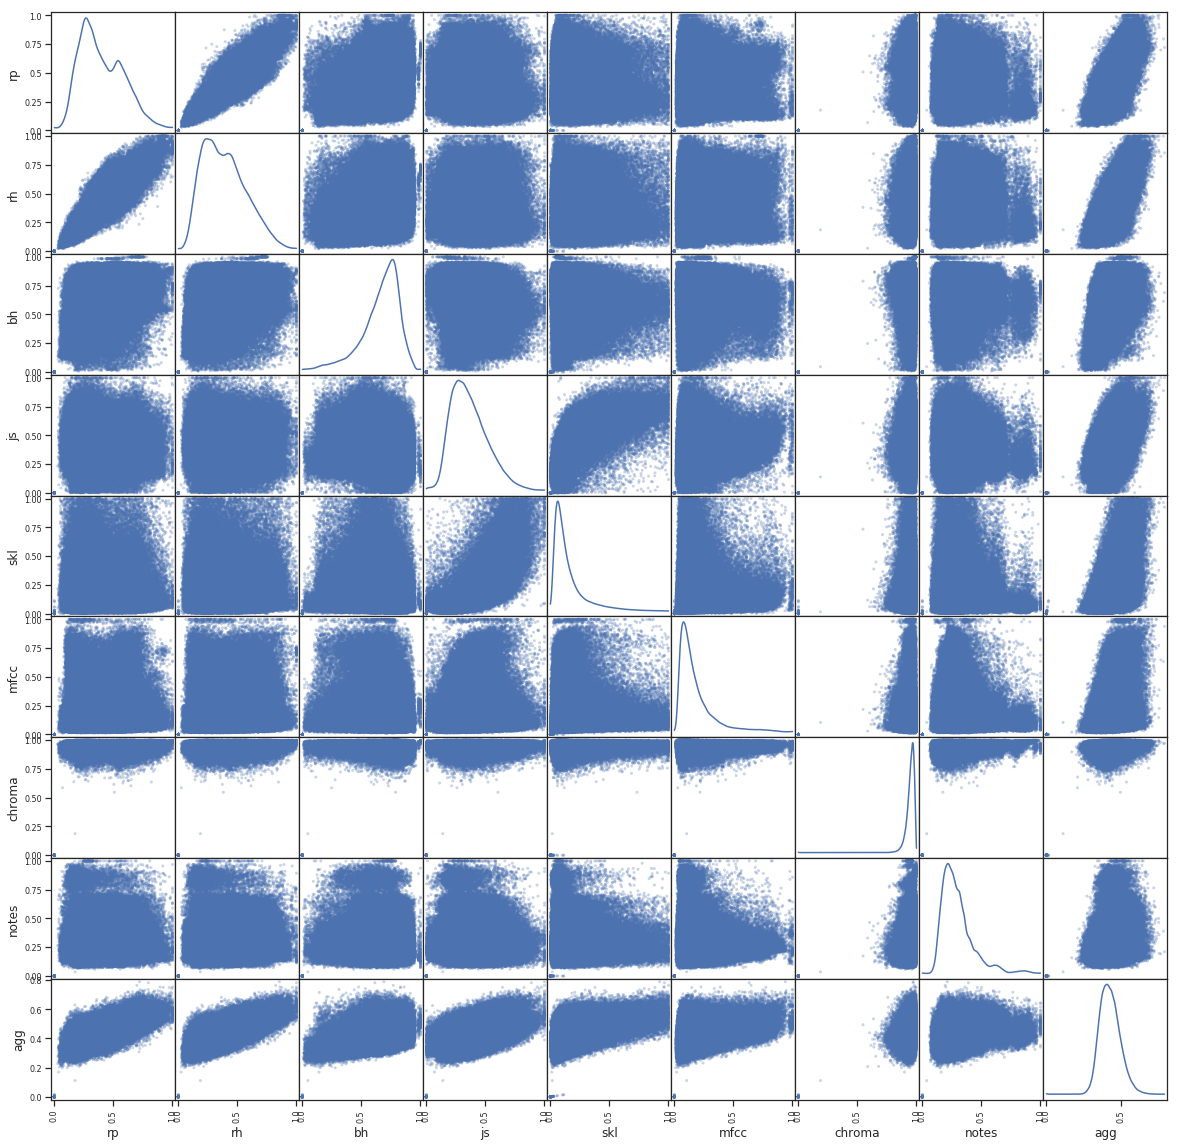
\includegraphics[scale=0.36]{Images/SparkFeat/scatter1517_KernelDensityEstimationHD.png}	
	}}
	\caption{correlation 95 songs, 19 genres (5 each), 1517 artists}
	\label{fig:corr3}
\end{figure}
\FloatBarrier

\subsection{Cover song identification}\label{covsongid}

\textit{\textbf{Able to find "Rock you like a Hurricane" cover as top recommendation in over 11500 songs\\}}
\ \\
\textit{\textbf{Able to find "Für Elise" cover as top recommendation in over 11500 songs, even with filter and refine\\}}
\ \\
\textit{\textbf{counting the hits in the top 10 results of 80 requested songs on 164 song dataset covers80:\\}}
\begin{itemize}
	\setlength\itemsep{-0.5em}
	\item chroma + notes + rp: 28
	\item chroma + notes: 24
	\item notes: 24
	\item notes + rp: 22
	\item mfcc + notes + rp: 20 (mfcc faulty)
	\item chroma: 16
\end{itemize}

\textit{interesting sidenote: results of chroma only and notes only different! Nearly ever}

\subsection{Genre similarity}\label{genrerec}

\textbf{\textit{\underline{100 Song Testset, 10 genres:\\}}} 
\begin{figure}[htbp]
	\centering
	\framebox{\parbox{1\textwidth}{ 			
			\begin{subfigure}{.495\textwidth}
				\centering    
				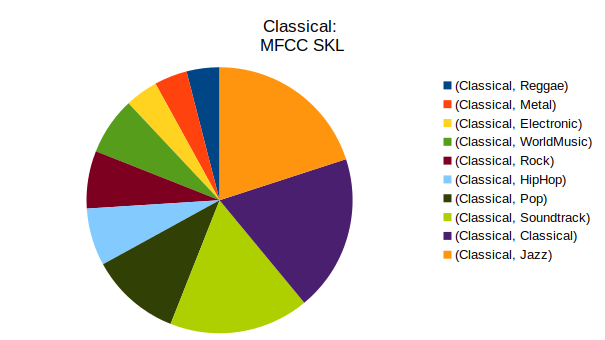
\includegraphics[scale=0.48]{Images/SparkFeat/Classical_MFCC_SKL.png}
				\caption{Classical - MFCC SKL}
				\label{cms}
			\end{subfigure}		
			\begin{subfigure}{.495\textwidth}
				\centering     
				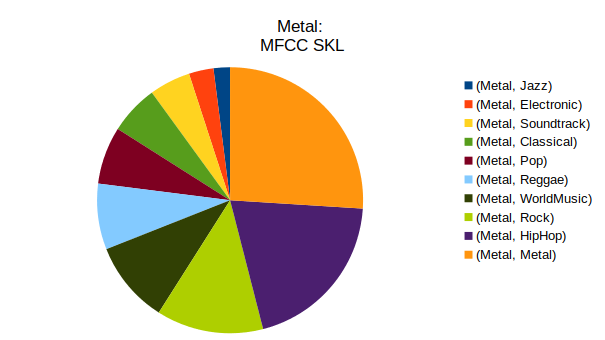
\includegraphics[scale=0.48]{Images/SparkFeat/Metal_MFCC_SKL.png}
				\caption{Metal - MFCC SKL}
				\label{mms}
			\end{subfigure}%	
			
			\begin{subfigure}{.495\textwidth}
				\centering    
				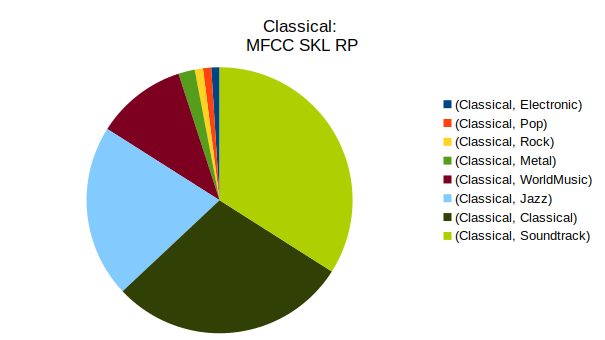
\includegraphics[scale=0.48]{Images/SparkFeat/Classical_MFCC_SKL_RP.png}
				\caption{Classical - MFCC SKL RP}
				\label{cmsr}
			\end{subfigure}
			\begin{subfigure}{.495\textwidth}
				\centering     
				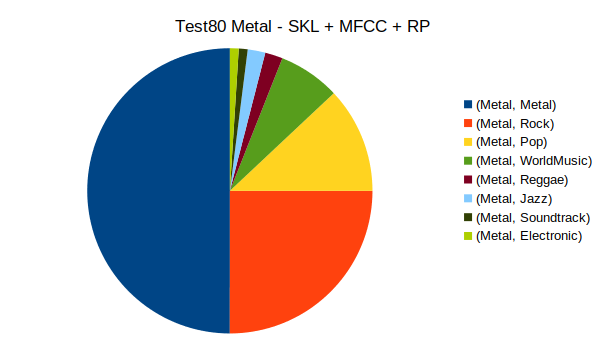
\includegraphics[scale=0.48]{Images/SparkFeat/Metal_MFCC_SKL_RP.png}
				\caption{Metal - MFCC SKL RP}
				\label{mfsr}
			\end{subfigure}%		
	}}
	\caption{genre recall 100 songs}
	\label{fig:genrerec}
\end{figure}


\noindent Scatter Matrix, 1 Song (Soundtack) from 100 song sample - distances, main diagonal = Kernel Density Estimation, picked subset of 5 genres in figure \ref{fig:corr8}
\begin{figure}[htbp]
	\centering
	\framebox{\parbox{1\textwidth}{ 			
			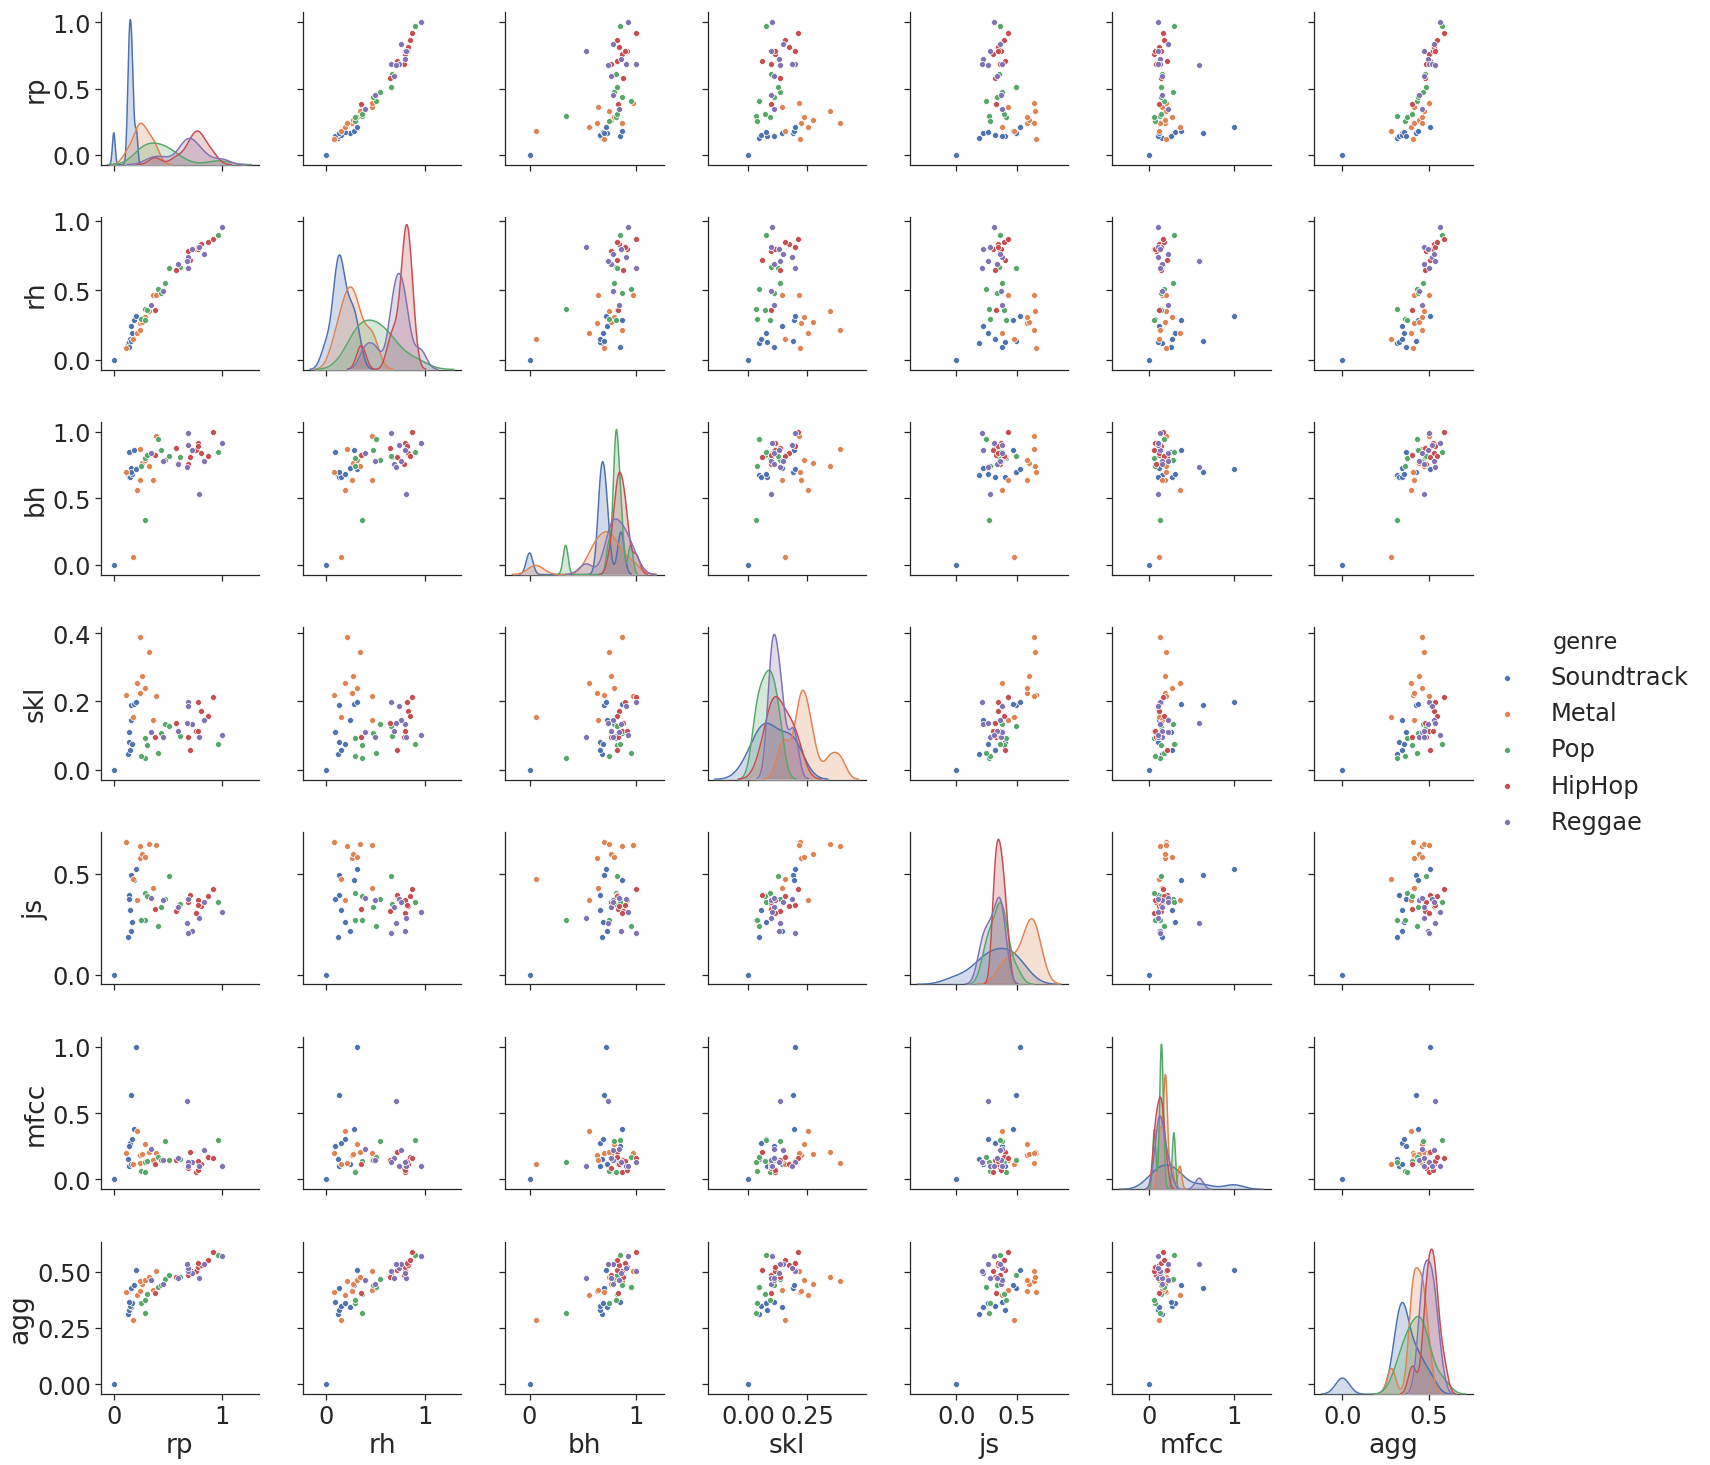
\includegraphics[scale=0.25]{Images/SparkFeat/soundtrack2.png}	
	}}
	\caption{distances 1 song (Soundtrack), 5 genres (10 songs each)}
	\label{fig:corr8}
\end{figure}

\noindent Scatter Matrix, 1 Song (Rock/ Metal) from 1517 artists - distances, main diagonal = Kernel Density Estimation, picked subset of 3 genres\\ All features combined recommends Rock primarily\\
Most interesting Detail: Plot JS - RP: overall similarity JS between Rock and Hip Hop - overall similarity RP between Classical and Metal - only one feature would not be able to separate all 4 genres in figure \ref{fig:corr5}
\begin{figure}[htbp]
	\centering
	\framebox{\parbox{1\textwidth}{ 			
			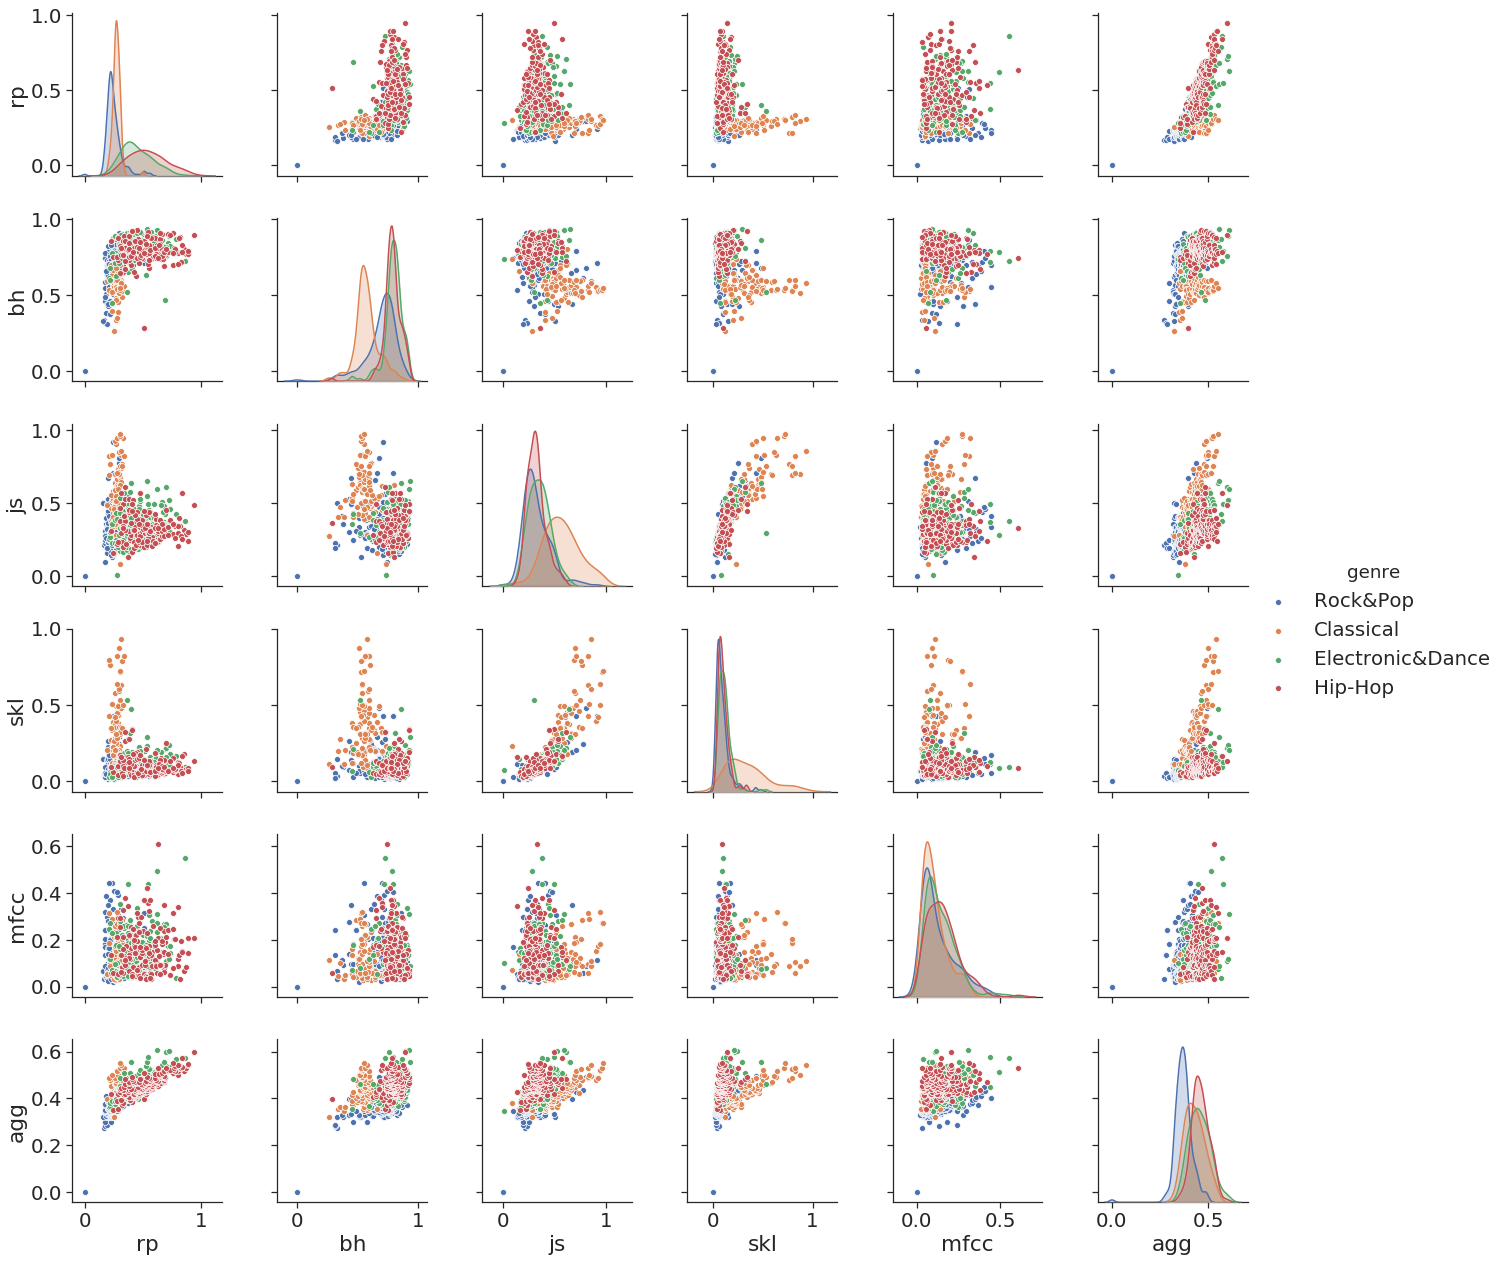
\includegraphics[scale=0.29]{Images/SparkFeat/rock.png}	
	}}
	\caption{distances 1 song, Rock/ Metal, 1517 artists, 4 genres}
	\label{fig:corr5}
\end{figure}

\noindent Scatter Matrix, 1 Song (Electronic) from 1517 artists - distances - figure \ref{fig:corr6}
No combination of features is able to accurately separate HipHop from Rock-Pop
\begin{figure}[htbp]
	\centering
	\framebox{\parbox{1\textwidth}{ 			
			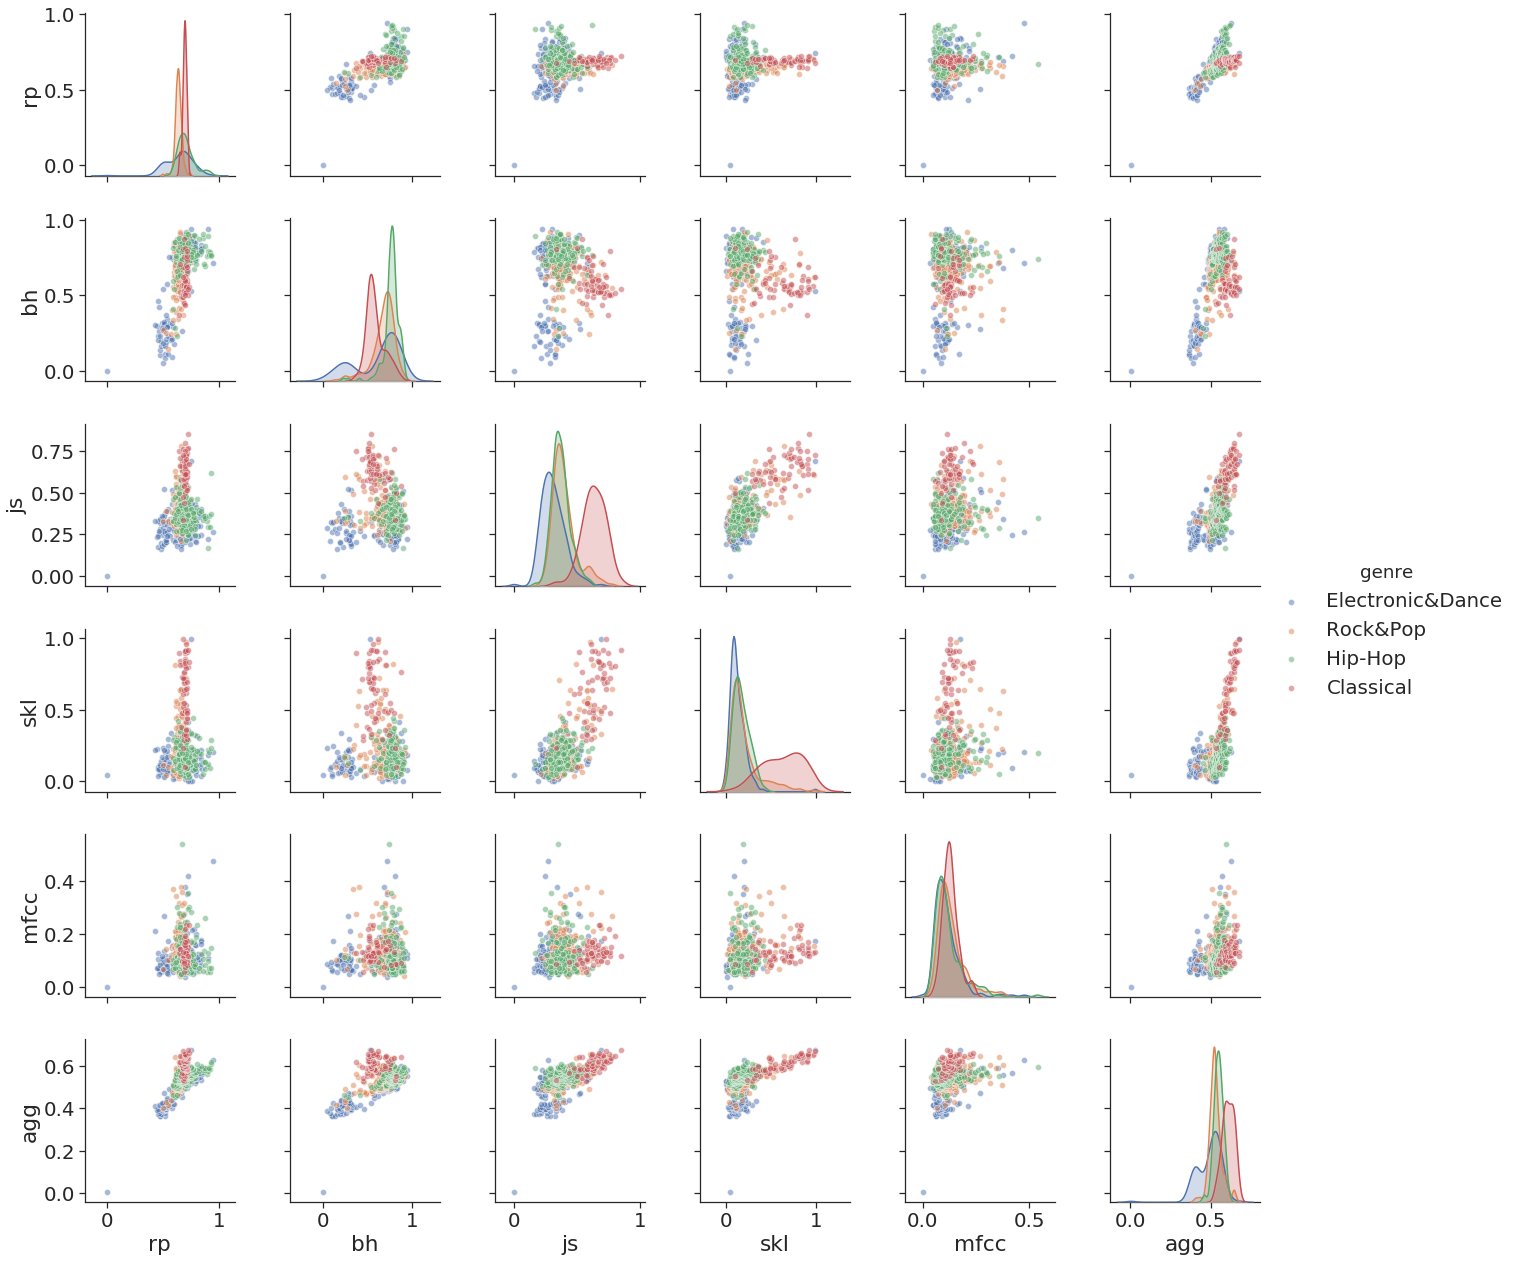
\includegraphics[scale=0.29]{Images/SparkFeat/electronic.png}	
	}}
	\caption{distances 1 song, electronic, 1517 artists, 4 genres}
	\label{fig:corr6}
\end{figure}
\FloatBarrier

\section{Subjective evaluation}

\subsection{Beyond genre boundaries}

\textit{\textbf{Rachmaninoff Prelude C\# minor full dataset Top 5 MFCC Euclidean\\}}
\\
Titel: Klassik/Rachmaninoff - Idil Biret - Op 3 No 2 Prelude in C - Sharp Minor
\begin{itemize}
	\setlength\itemsep{-0.5em}
	\item Klassik/Rachmaninoff - Piano Concerto No2 In C Minor Op18-1 Moderato
	\item Klassik/Liszt - Piano Concerto No 1 in E flat major S124(LWH4) Allegro maestoso
	\item Klassik/Brahms - Piano Sonata No2 in F sharp minor Op2 - III Scherzo allegro
	\item \underline{Metal\&Rock/Steve Moore - Intro \& Credits}
	\item Klassik/Liszt - Piano Concerto No 1 in E flat major S124(LWH4) Allegro animato
\end{itemize}

\subsection{Honorable mentions}

\section{Summary and outlook}

In the first part of this thesis an overview over the field of MIR was given, different audio features were explained, similarity measurements evaluated and multiple algorithms for timbre similarity were presented.\\
Data was collected, over 1TB of music data, 114000 songs. The necessary audio features were extracted and pre-processed (Melody Estimation) in parallel using MPI on a cluster paving the way for usage with big data processing frameworks.\\
The features were loaded into the HDFS of a cluster and multiple similarity measurements were implemented, tested, evaluated and improved. With spark multiple approaches (RDD, DataSet, Filter and Refine, Cluster Configurations) were tested.\\
The results were presented and visualized.\\
\ \\
outlook:\\
\ \\
more state of the art similarity (blocked)\\
performance improvements\\
spark streaming, real-time\\
jensen-shannon investigation\\
garbage collecting issue\\
Genre and metadata, Genre specific features, combinations and variable model, Collaborative Filtering, Lyrics\\
reduce hubness\\

%\addtolength{\textheight}{-12cm}   % This command serves to balance the column lengths
% on the last page of the document manually. It shortens
% the textheight of the last page by a suitable amount.
% This command does not take effect until the next page
% so it should come on the page before the last. Make
% sure that you do not shorten the textheight too much.